
\section{DAG Traversal Algorithm}\label{apx:DAG-algo}
The Query Manager is presented with a DAG for each query, where each
node in the DAG represents a relational operator primitive.
The edges in the DAG are annotated with whether the 
\textit{consumer} operator is blocked on the output produced 
by the \textit{producer} operator, or whether data pipelining is
allowed between two adjacent operators. 

Consider a sample join query and its DAG showed in Figure~\ref{fig:dag}.
The solid arrows in the DAG correspond to ``blocking'' dependencies,
and the dashed arrows indicate pipeline-able/non-blocking dependencies. 
To execute this query we need to select tuples from the \verb+ddate+ 
table, stream them to a hash table, which can then be probed by tuples that are 
created by the selection operator on the \verb+lineorder+ table. %(i.e. match the predicate on that table). 
The output of the probe hash operation can be sent to the print operator, which
displays the result. % tuples. 
Note that the ``drop hash'' operator is used to drop the hash table, but only 
after the ``probe hash'' operation is complete. 
Similarly, the other drop operators indicate when intermediate data can be deleted. 

\begin{algorithm}
	\caption{DAG Traversal}
	\begin{algorithmic}[1]
		\State G = \{V, E\}
		\State activeEdges = \{e $\in$ E $|$ e.isNotPipelineBreaking()\}
		\label{alg:pipelining}
		\State inactiveEdges = \{e $\in$ E $|$ e.isPipelineBreaking()\}
		\State completedNodes = \{\}
		
		\For {v $\in$ V}:
			\If {v.allIncomingEdgesActive()}
				\State v.active = True
			\Else
				\State v.active = False
			\EndIf
		\EndFor
		
		\While {completedNodes.size() $<$ V.size()}
		\For {v $\in$ V -- completedNodes}
		\If {v.allIncomingEdgesActive()}
			\State v.active = True \label{alg:depMet}
		\EndIf
		\If {v.active}
		\State v.getAllNewWorkOrders() \label{alg:getWork}
		\If {v.finishedGeneratingWorkOrders()} \label{alg:finishGenWork}
		\State completedNodes.add(v) \label{alg:nodeComplete}
		\For {outEdge $\in$ v.outgoingEdges()}
		\State activeEdges.add(outEdge)\label{alg:outEdgesActive}
		\EndFor
		\EndIf
		\EndIf
		\EndFor	
		\EndWhile
	\end{algorithmic}
	\label{alg:dag-traversal}
\end{algorithm}

\begin{figure}[]
	\centering
	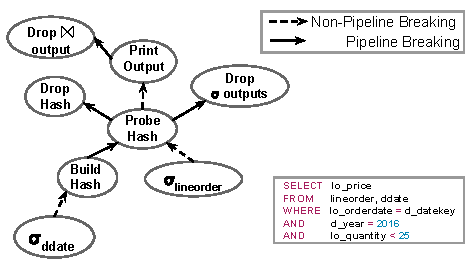
\includegraphics[width=\columnwidth]{policy/figures/QueryPlan.pdf}
	\vspace*{-2em}
	\caption{\textbf{A join query and its DAG}}
	\label{fig:dag}
%	\vspace*{-1.5em}
\end{figure}

The Query Manager uses a DAG Traversal algorithm (cf. Algorithm~\ref{alg:dag-traversal}) to process the DAG, which essentially is an iterative graph traversal method. 
The algorithm simply finds nodes in the DAG that have all their dependencies met, and marks such nodes as ``active'' (line~\ref{alg:depMet}).
Work orders are requested and scheduled for all active nodes (line~\ref{alg:getWork}), and 
the completion of work orders is monitored. 
Operators are stateful and they produce work orders when they have the necessary data.
The work order generation stops (line~\ref{alg:finishGenWork}) when the operators no longer have any input to produce additional work orders.
When no more work orders can be generated for a node, that node is marked as 
``completed'' (line~\ref{alg:nodeComplete}). 
When a node is marked as completed, all outgoing blocking edges (the solid lines 
in Figure~\ref{fig:dag}) are ``activated'' (line~\ref{alg:outEdgesActive}). 
Pipelining is achieved as all non-blocking edges (dotted lines in 
Figure~\ref{fig:dag}) are marked as active upfront (line~\ref{alg:pipelining}).
The query is deemed as completed when all nodes are marked as ``completed.''

% Note(harshad) - The DAG traversal example seems to be taking lots of space and can be omitted, as it diverts the attention away from the meat of the paper. 
%\subsubsection{DAG Traversal Example}\label{sssec:dag-traversal-example}
%To illustrate the execution of the scheduler algorithm, consider the 
%DAG shown in Figure~\ref{fig:dag}.
%Initially, only the two selection relational operators (shown in the DAG using
%the symbol $\sigma$) are \textit{schedulable}.\footnote{Initially, the print 
%operator is \textit{active} too, but as there's no input available, it can't
%produce any work order.}
%So, the Query Manager generates work orders for these operators. 
%In this case, there is one work order for each input block in each of the two
%input relations.\footnote{To avoid both select operators from being co-scheduled
%concurrently, a dependency link can be created between these two operators.
%Thus, work on the select operator on the $\mathtt{lineorder}$ table is started
%only after the select operator on the $\mathtt{ddate}$ table has completed. 
%Such decisions are made by the optimizer.}
%
%The Foreman assigns these work orders to the available worker threads. 
%The worker threads execute the operations specified in the work orders. 
%Note that given the independent block design (see Section~\ref{ssec:storage-manager}) 
%it is possible that two work orders on the same table may invoke different code paths. 
%For example one block on the \verb+ddate+ table may have an index sub-block on 
%the \verb+d_year+ attribute, and this index may be chosen to evaluate the tuples 
%in that block. 
%Another block on that same \verb+ddate+ table may not have any indices, and so 
%the selection operation for tuples in that second sub-block may resort to a simple scan. 
%In addition, the operator algorithm may choose to make a local decision on which 
%access plan to use. 
%So, e.g. even if each data block in the \verb+ddate+ table has an index 
%of the \verb+d_year+ attribute some work orders may use the index and others may 
%not. (The optimization algorithm for making these local decisions is beyond the 
%scope of this paper.)
%Essentially, the scheduler is largely oblivious to how the work orders are executed 
%and there is no global recipe that is imposed on the work orders that correspond 
%to a node in the DAG.
%
%Work orders may produce output data that are stored in blocks in the buffer pool. 
%In the case of the query in Figure~\ref{fig:dag}, the selection work orders on the \verb+ddate+
%table insert the selected tuples into data blocks that correspond to a new 
%temporary table. 
%%(the execution of the work orders is vectorized for efficiency). 
%These data blocks are pipelined to the next stage.\footnote{There is a 
%mechanism to allow multiple concurrent work orders from the same
%operator in the DAG to insert into a common output/temporary data
%block to avoid block internal fragmentation, and to facilitate early 
%pipelining. We omit these details.}
%In other words, as soon as there is a full block of tuples from applying the 
%selection operator on the \verb|ddate| table, a work order is created for the 
%\textit{build hash} operator. (Notice that the edge connecting the selection
%operator and the build hash operator permits data pipelining.)
%
%To begin the probe phase of the hash join, the building of the hash table must be 
%complete, as there is a pipeline-breaking dependency between the probe operator 
%and the build operator. 
%Thus, the DAG traversal algorithm only marks the probe hash operator node as 
%active when the build hash operator has completed. 
%Results from probing the hash table can be immediately pipelined to the print 
%operator.
%The drop operators ensure that intermediate data is dropped before the query is 
%deemed to have completed. 

\section{Resource Map Discussion}\label{apx:resource-map}
An example Resource Map of an incoming query to the system is shown below:
\begin{lstlisting}[language=python, 
								   basicstyle=\ttfamily\small, 
								   showstringspaces=false,
								   keywordstyle=\color{bondiblue}\bfseries, 
								   emph={CPU, Memory}, 
								   emphstyle=\color{cardinal}\bfseries]
CPU:    {min: 1 Core, max: 20 Cores}
Memory: {min: 20 MB,  max: 100 MB}
\end{lstlisting}

This Resource Map states that the query can use 1 to 20 cores (i.e. specifies the range of intra-operator parallelism) and is estimated to require a minimum of 20 MB of memory to run, and an estimated 100 MB of memory in the worst case.

In \sys{}, the query optimizer provides the estimated memory requirements for a given query.
Other methods can also be used, such as inferring the estimated resources from the previous runs of the query or other statistical analyses.
The scheduler is agnostic to how these estimates are calculated.

\section{Pipelining in \sys{}}\label{apx:pipelining}
During a work order (presumably belonging to a producer relational operator in a pipeline) execution, output data may be created (in blocks in the buffer pool). 
When an output data block is filled, the worker thread sends a ``block filled'' message to the corresponding query's manager via the following channel: Worker $\rightarrow$ Foreman $\rightarrow$ Policy Enforcer $\rightarrow$ Query Manager.
The Query Manager may then create a new work order (for a consumer relational operator in the pipeline) based on this information;
e.g. if this block should be pipelined to another operator in the query plan.

Note that pipelining in \sys{} works on a block-basis, instead of the traditional tuple-basis.

\section{Motivation for the Learning Agent Module}\label{apx:learning-motivation}
One might question the need of the Learning Agent and instead consider assigning a fixed probability value to each query (say $1/N$, with $N$ queries in the fair policy).
In the following section, we address this issue. 
A motivational example for the learning agent is described in Appendix~\ref{apx:learning-motivation}.

We perform an experiment, where the goal is to analyze the patterns in work order execution times of two queries. 
The dataset used for the experiment comes from the Star Schema Benchmark (SSB)~\cite{ssb} 
at a scale factor of 100. %(c.f. Section~\ref{ssec:workload} for benchmark details).
We pick two SSB queries $Q1.1$ and $Q4.1$, and execute them on a machine with 40 CPU cores. 
$Q1.1$ has a single join operation and $Q4.1$ has four join operations.
Figure~\ref{fig:q1.1-q4.1-time-per-wo} shows the observed average time per work order for both queries.
We now describe the trends in time per work order for the queries.

We can observe $Q1.1$'s execution pattern denoted by the dashed line in Figure~\ref{fig:q1.1-q4.1-time-per-wo}. 
The time per work order remains fairly stable (barring some intermittent fluctuations) from the beginning until 1.8 s.
This phase corresponds to the selection operation in $Q1.1$ which evaluates predicates on the \textit{lineorder} (fact) table.
A small bump in time per work order can be observed at the 1.8 s mark, when the probe phase of $Q1.1$ begins and continues until 2 s.
Towards the end of the execution of $Q1.1$, (2.2 s) there is a spike in time per work order when the query enters the aggregation phase. 
The output of the hash join is fed to the aggregation operation. 
The results of aggregation are stored in per-thread private hash tables, which are later merged to produce the final output.

\begin{figure}[h]
	\centering
	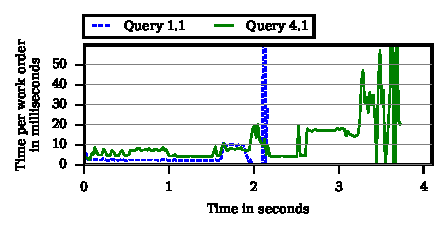
\includegraphics[width=\columnwidth]{policy/figures/q11-q41-time-per-wo.pdf}
	\vspace{-2.5em}
	\caption{\textbf{Time per work order for SSB Q1.1 and Q4.1}}
	\label{fig:q1.1-q4.1-time-per-wo}
%	\vspace{-2em}
\end{figure}

Now we analyze the execution pattern for $Q4.1$ which has 4 join operations. 
This query is more complex than $Q1.1$.% which has a single join.
%Due to the more complex nature of the query, 
Therefore, the execution pattern of $Q4.1$ exhibits more phases, with different times per work order as compared to $Q1.1$.
Various small phases before the 0.5 s mark correspond to the selection predicates that are applied to the dimension tables. (Note that in $Q4.1$ there is no selection filter on the \textit{lineorder} table).
The selections on dimension tables get executed quickly.
The longer phases denote the different probe hash table operations in the query.
Towards the end, similar to $Q1.1$, there is a spike in the execution time per work order which correspond to the aggregation phase.

It is clear that the work order execution times for both queries are different, and the difference between them changes over time. 
If the scheduler assigns the same probability to both queries (i.e. 0.5), it is equally likely to schedule a work order from either of them. 
As a result, the queries will have different CPU utilization times in a given epoch, thus resulting in an unfair CPU allocation. 
In order to be consistently fair in allocating CPU resources to the queries, we should continuously observe the work order execution times of queries and adjust the CPU allocation accordingly. 

\section{Usage of Linear Regression in Learning Agent}\label{apx:linear-regression-usage}
The Learning Agent uses linear regression for predicting the execution time of the future work orders.
To lower the CPU and memory overhead of the model, we limit the amount of execution statistics stored in the Learning Agent.
We discard records beyond a certain time window. 
When all the work orders of an operator finish execution, we remove its records completely. 
In a query, if multiple relational operators are active, linear regression combines the statistics of all active operators and predicts a single value for the next work order execution time.

\section{Resource Choices for Policy Implementations and Load Controller Implementations}\label{apx:resource-discussion}
In the current implementation of \sys{}, we have focused on two key types of resource in the in-memory deployment scenarios -- CPU and memory. 
Both these resources have different resource characteristics, which we outline below.

First, consider the CPU resource. 
On modern commodity servers there are often tens of CPU cores per socket, and the aggregate number of cycles available per unit time (e.g. a millisecond) across all the cores is very large. 
Further, an implication of \sys{}'s fine-grained task allocation and execution paradigm is that the CPU resource can be easily shared at a fine time-granularity. 
Several work orders, each from different query can be executed concurrently on different CPU cores, and each query may execute thousands or millions or even more number of work orders. 
Thus, in practical terms, the CPU resource can be viewed as a nearly infinitely divisible resource across concurrent queries. 
In addition, overall system utilization is often measured in terms of the CPU utilization. Combining all these factors, specifying a policy  in terms of the CPU utilization is natural, and intuitive for a user to understand the policy. 
For example, saying that a fair policy equally distributes the CPU resource across all (admitted) concurrent queries is simple to understand and reason. 

Memory, on the other hand, is a resource that is allocated by queries in larger granular chunks. 
Active queries can have varying memory footprints (and the footprint for a query can change over the course of its execution). 
Thus, memory as a resource is more naturally viewed as a ``gating'' resource. 
Therefore, it is natural to use it in the load controller to determine if a query can be admitted based on its requested memory size. 
Actual memory consumption for queries can also be easily monitored, and when needed queries can be suspended if memory resource needs to be freed up (for some other query, perhaps with a higher priority). 

\section{Applicability of SSB for our evaluation}\label{apx:ssb}
The SSB is based on the TPC-H benchmark, and is designed to measure the query performance when %database systems in support of classical 
the data warehouse uses the popular Kimball~\cite{Kimball} approach. 
At a scale factor of X, the benchmark corresponds to about X GB of data in the 
corresponding TPC-H warehouse.
The SSB benchmark has 13 queries, divided in four categories. 
Each query is identified as \textbf{qX.Y}, where $X$ is the class and $Y$ is the query 
number within the class.
There are four query classes, i.e. $1\leq X\leq4$. 
The first and second classes have three queries each, the third class has four queries, and 
the fourth class has three queries.
The queries in each category are similar with respect to aspects such as the 
number of joins in the query, the relations being joined, the filter and aggregation 
attributes. 
The grouping of queries in various classes makes this benchmark suitable for our 
experiments, as it provides a way of assigning priorities to the queries based on their class. 

\section{Policy Enforcer}\label{apx:policy-enforcer}
The Policy Enforcer applies a high level policy for resource allocation among concurrent queries. 
It uses a probabilistic-framework to select work orders from a pool of work orders 
belonging to different concurrent queries for scheduling. 
The Policy Enforcer assigns a probability to each active query, which indicates the likelihood of a work order from that query getting scheduled for execution in the near future. 
The probability-based work order selection strategy brings powerful control to the scheduler through a single parameter -- i.e. by controlling the probability 
setting, the scheduler can control the resource sharing among concurrent queries. 
%A work order from a query with higher probability is more likely to get scheduled 
%than a work order from a query with lower probability. 

The challenge in designing the policy enforcer lies in transforming the policy specifications to a set of probabilities. 
A critical piece that we use in such transformations is the prediction of work order 
execution times for the concurrent queries, which is done by the Learning Agent. 
%described in Section~\ref{ssec:learning}. %and depicted in Figure~\ref{fig:scheduler-cycle}.
In the remainder of this section, we provide an intuition for deriving probability values from the work order execution times. 
%A formal model for the probability computations for different policies is presented in Section~\ref{sec:policy}.

\begin{figure}[]
	\centering
	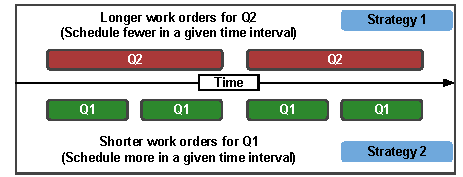
\includegraphics[width=\columnwidth]{policy/figures/Probability-explanation.pdf}
	\vspace{-2em}
	\caption{\textbf{Scheduling queries having different work order execution times for the fair policy. The solid boxes with $Q_{i}$ depicts the lifetime of a work order from the Query $Q_{i}$}}
	\label{fig:probability-explanation}
	%	\vspace{-1.5em}
\end{figure}

We now motivate the probabilistic approach used by the Policy Enforcer with an example.
Consider a single CPU core and two concurrent queries $q_{1}$ and $q_{2}$. 
(The idea can be extended to multi-cores and more than two queries.)
Initially, we assume perfect knowledge of the execution times of work orders of the queries. 
Later, we will relax this assumption. 

Let us assume that as per the policy specifications, in a given time interval, the CPU resources should be shared equally. 
Suppose that work orders for $q_{1}$ take less time to execute than work orders for 
$q_{2}$, as shown in Figure~\ref{fig:probability-explanation}.
As the Policy Enforcer aims to allocate equal share of the CPU to $q_1$ and $q_2$, a simple strategy can be to schedule proportionally more work orders of $q_{1}$  than those of $q_{2}$, in a given time window. 
The number of scheduled work orders is inversely related to the work order execution 
time. 
This proportion can be determined by the probabilities $pb_{1}$ and $pb_{2}$ for queries $q_1$ and $q_2$, respectively.
The probability $pb_i$ is the likelihood of the scheduler scheduling next work order from query $i$. 
The probability is assigned by the Policy Enforcer to each active query in the system.
Note that, $pb_{1} > pb_{2}$ and $pb_{1} + pb_{2} = 1$.

%Such strategy will result in similar \textit{CPU occupancy} with respect to time 
%for both the queries, thereby fairly sharing the CPU resource in a given time 
%frame.  If the policy enforcer keeps scheduling the work orders similarly for the rest of 
%the  workload execution, it is easy to see that the queries will share the CPU 
%\textit{fairly}, as demanded by the policy. 

Notice that the Policy Enforcer is not concerned with the complexities of the operators in the query DAGs. 
It simply maintains the probability associated with each active query which is determined by the query's predicted work order execution times.

The Policy Enforcer can also function with workloads that consist of queries categorized in multiple classes, where each class has a different level of ``importance'' or ``priority''. 
The policy specifies that the resource allocation to a query class must simply be in accordance to its importance, i.e. queries in a more important class should collectively get a higher share of the resources, and vice versa.
In such scenarios, the Policy Enforcer splits its work order selection strategy in two steps - selection of a query class and subsequent selection of a 
query within the chosen query class.
Intuitively, the Policy Enforcer should assign higher probability to the more 
important class and lower probability to the less important class.

Once a query class is chosen, the Policy Enforcer must pick a query from the chosen class. 
Each query class can specify an optional intra-class resource allocation sub-policy. 
By default, all queries within a class are treated equally.
Thus, the probability-based paradigm can be used to control both inter and intra-class resource allocations.

There could be many reasons for categorizing queries in classes, including the need to associate some form of urgency (e.g. interactive vs batch queries), or marking the importance of the query source 
(e.g. the position of the query submitter in an organizational hierarchy). 
In addition, the resource allocations across different classes can also be chosen based on various scales, such as linear or exponential scale allocations based on the class number. 
An attractive feature of the Policy Enforcer is that it can be easily configured for use in a variety of ways.
Under the covers, the Policy Enforcer simply maps each class to a collective class probability value, and then maps each query in each class to another probability. 
Once these probabilities are calculated, the remaining mechanisms simply use them to appropriately allocate resources to achieve the desired policy goal.
